\documentclass{article}
\usepackage{afterpage}
\usepackage{float}
\usepackage{longtable}
\usepackage{graphicx}
\usepackage{pdflscape}
\usepackage[numbers,sort&compress]{natbib}
\usepackage{psfrag}

\usepackage{amsmath}
\usepackage{amsfonts}
\usepackage{graphicx}
\usepackage{nicefrac}
\usepackage{graphicx}
\usepackage{caption}
% \usepackage{subcaption}
\usepackage{subfigure}
% \usepackage{algorithm}
% \usepackage{paralist}
% % \usepackage[geometry]{ifsym}
\usepackage{rotating}
%
\usepackage{listings}
\usepackage{xcolor}
\lstset{language=C++,
                keywordstyle=\color{blue},
                stringstyle=\color{red},
                commentstyle=\color{green},
                morecomment=[l][\color{magenta}]{\#}
}
\begin{document}


\subsection*{Gradient matrix}

Construction of the discrete gradient matrix $C$ is done using the C++ interface of FEniCS to increase the speed.

\begin{itemize}
    \item $A$: Discrete curl-curl
    \item $M$: Mass matrix Nedelec elements
    \item $B$: Gradient matrix
    \item $L$: Laplacian matrix on scalar space
\end{itemize}


\begin{table}[h!]
\centering
    \begin{tabular}{ccccc}
    \hline
      l &  DoF &        $AC$ &    $MC-B^T$ &      $BC-L$ \\
    \hline
      1 &     16 &  0.0000e+00 &  1.5543e-15 &  4.4409e-16 \\
      2 &     56 &  0.0000e+00 &  1.5543e-15 &  4.4409e-16 \\
      3 &    208 &  0.0000e+00 &  1.5543e-15 &  4.4409e-16 \\
      4 &    800 &  0.0000e+00 &  1.5543e-15 &  4.4409e-16 \\
      5 &   3136 &  0.0000e+00 &  1.5543e-15 &  4.4409e-16 \\
      6 &  12416 &  0.0000e+00 &  1.5543e-15 &  4.4409e-16 \\
      7 &  49408 &  0.0000e+00 &  1.5543e-15 &  4.4409e-16 \\
    \hline
    \end{tabular}
    \caption{Max element of matrix}
    \label{tab:awesome_image}
\end{table}

To check the the construction of the $C$ matrix is correct I checked the three identities in your 07 paper.



\subsection*{Edge to nodal grid operator}

Construction of the grid transfer operator $P$ is done using the C++ interface of FEniCS to increase the speed. Left to right in Figure~\ref{fig:awesome_image}:
\begin{itemize}
    \item[LEFT: ] $Px*\mbox{nodal values of sin(x}) \ \ $  as a Nedelec function
    \item[MIDDLE: ] $Py*\mbox{nodal values of sin(x}) \ \ $ as a Nedelec function
    \item[RIGHT: ] $\mbox{nodal values of sin(x}) \ \ $ as a nodal Lagrange function
\end{itemize}

\begin{figure}[h!]
    \centering
    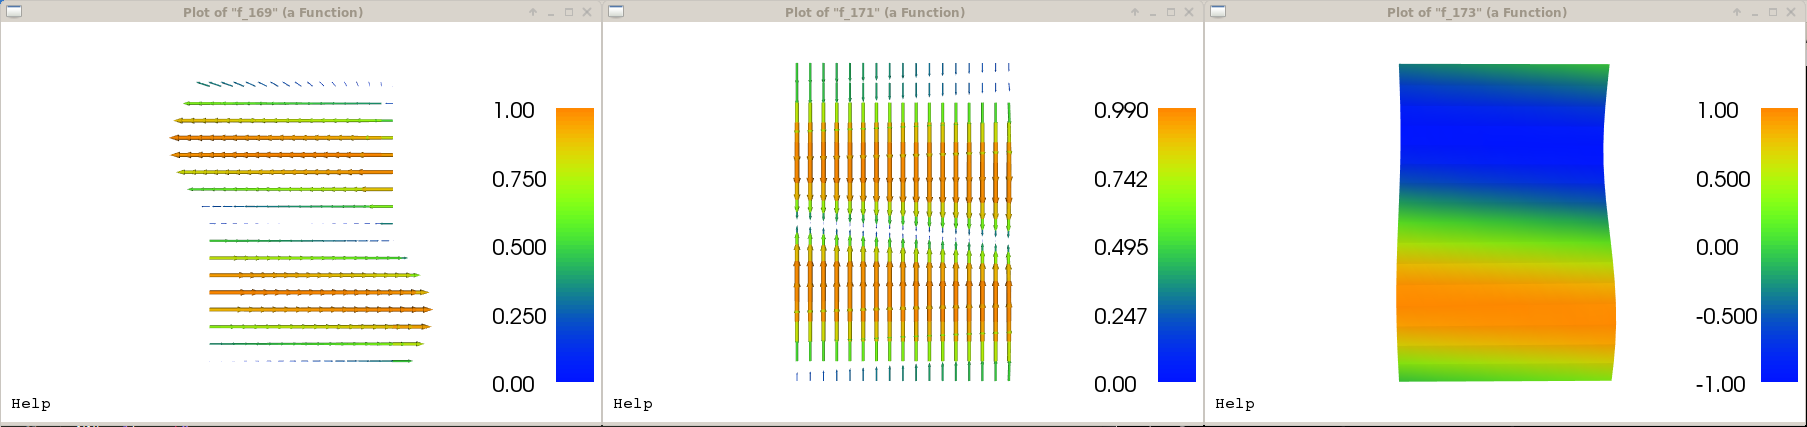
\includegraphics[width=1\textwidth]{Figures/Interpolation.png}
    \caption{}
    \label{fig:awesome_image}
\end{figure}



\subsection*{Construction of $C$ and $P$}

Small C++ code sample of how the $C$ and $P$ matrices are formed.
\begin{itemize}
    \item \tt{dataX}: values of $P_x$
    \item \tt{dataY}: values of $P_y$
    \item \tt{dataZ}: values of $P_z$
    \item \tt{data}: values of $C$
    \item \tt{column}: column index
    \item \tt{row}: row index
\end{itemize}
\begin{lstlisting}
for (int i = 0; i < m; ++i) {
    k = k + 1;
    dolfin_edge = new Edge(mesh, i);
    const uint* edgeVERTICES = dolfin_edge->entities(0);


    dataX[k]=0.5*dolfin_edge->length()*Ntangent[0];
    dataY[k]=0.5*dolfin_edge->length()*Ntangent[1];

    if (dim == 3) {
        dataZ[k]=0.5*dolfin_edge->length()*Ntangent[2];
    }
    data[k] = 1;
    row[k] = i;
    column[k] = edgeVERTICES[1];

    k = k + 1;
    dataX[k]=0.5*dolfin_edge->length()*Ntangent[0];
    dataY[k]=0.5*dolfin_edge->length()*Ntangent[1];

    if (dim == 3) {
        dataZ[k]=0.5*dolfin_edge->length()*Ntangent[2];
    }
    data[k] = -1;
    row[k] = i;
    column[k] = edgeVERTICES[0];
}
\end{lstlisting}

I do not really pay attention to the orientation of the cells with respect to the Nedelec degrees of freedom but from Dan's code she seems not to pay attention to this either.... From the the test that I have done to check $C$ and $P$ the orientation does not seem to matter....

\subsection*{Trilinos Results}

Here are some $3D$ results using PyTrilinos on a regular grid. For the Trilinos example all you need to supply is the gradient matrix . I am in contact with the people at Trilinos to figure out what is wrong with the code as it does not seem to yield scalable results.....

\begin{tabular}{lrrrr}
\hline
 l &   DoF &   Solution  Time &  Iterations \\
\hline
 3 &     4,184 &   0.0445 &           3 \\
 4 &    31,024 &   0.5140 &           5 \\
 5 &   238,688 &   7.2629 &           9 \\
 6 &  1,872,064 &  98.5120 &          15 \\
 7 & 14,827,904 & 1120.0655 & 21\\
\hline
\end{tabular}


\subsection*{Petsc Results}

Here are some $2D$ results using Petsc on a regular grid. Here we require the construction of the $P$ matrix. The application of the precondition is given by
$$P_{\mbox{curl}}^{-1} = diag(A+M)^{-1} + P (\textbf{L}_{\mbox{N}}+\textbf{Q}_{\mbox{N}})^{-1}P^T+CL^{-1}C^T$$
In Hiptmair and Xu's paper it is unclear where boundary conditions need to be applies to $\textbf{L}_{\mbox{N}}+\textbf{Q}_{\mbox{N}}$ and $L$. I have pulled out the two sections of the paper that talk about these matrices
\subsubsection*{Shifted vector Laplacian}
\begin{figure}[h!]
    \centering
    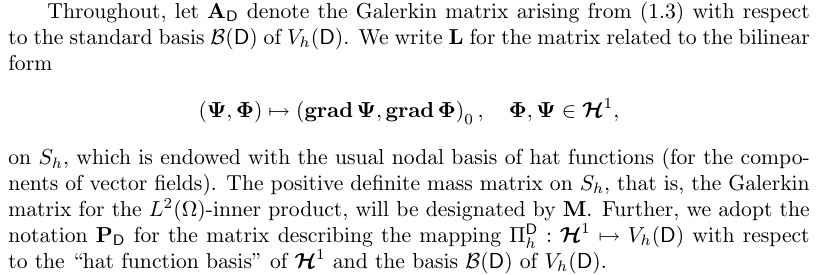
\includegraphics[width=1\textwidth]{Figures/VectorLaplacian.png}
    \caption{}
    \label{fig:121}
\end{figure}

\subsubsection*{Scalar Laplacian}

\textcolor{white}{2}
\begin{figure}[h!]
    \centering
    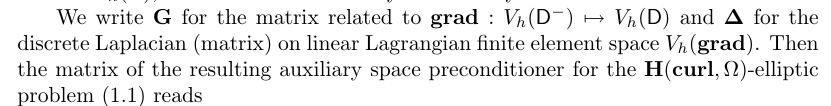
\includegraphics[width=1\textwidth]{Figures/ScalarLaplacian.png}
    \caption{}
    \label{fig:121}
\end{figure}


I have looked closely at Dan's code and she does not seem to apply boundary conditions to $\textbf{L}_{\mbox{N}}+\textbf{Q}_{\mbox{N}}$ and $L$ either.



Running the code produces the table below.

\begin{tabular}{lrrrr}
\hline
  l &  B DoF &    Time &  Iterations \\
\hline
1 &     16 &  0.0050 &          12 \\
2 &     56 &  0.0083 &          21 \\
3 &    208 &  0.0176 &          39 \\
4 &    800 &  0.0423 &          61 \\
5 &   3136 &  0.1365 &          87 \\
6 &  12416 &  0.7172 &         140 \\
7 &  49408 &  5.3862 &         218 \\
\hline
\end{tabular}


The results show even less scalability than with the Trilinos code.

\subsection*{Questions/comments}

\begin{itemize}
    \item Do $\textbf{L}_{\mbox{N}}+\textbf{Q}_{\mbox{N}}$ and $L$ require boundary conditions?
    \item Do I create $L+Q$ on the scalar space and apply the inverse 2 or 3 times depending on the spacial of the problem? This is what Dan does in her code..
    \item Performed the same test on the gradient matrix $C$ and interpolation operator $P$ on unstructured meshes and they also produce the expected results
    \item Checked that default BoomerAMG settings for $\textbf{L}_{\mbox{N}}+\textbf{Q}_{\mbox{N}}$ and $L$ produce iterations that are independent of the mesh size
    \item I have check symmetric Gauss-Seidel sweep instead of the Jacobi iterations for $A+M$ but it does not seem to improve scalability. Also, have applied damped Jacobi as well as a few iterations but neither seem to help much.
    \item I have combed through Dan's code to check that I'm doing things right and I can't really find a difference in what I'm doing compared to her.....
    \item Used the approach in PARALLEL AUXILIARY SPACE AMG FOR H(curl) PROBLEMS by Tzanio V. Kolev and Panayot S. Vassilevski to construct the interpolation matrix to check it gives the same matrix as from your Paper (see Figure~\ref{fig:in})
    \begin{figure}[h!]
    \centering
    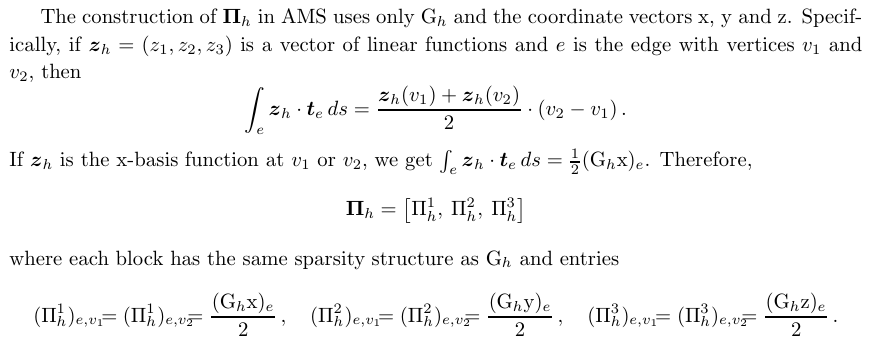
\includegraphics[width=1\textwidth]{Figures/InterpolationConstruct.png}
    \caption{}
    \label{fig:in}
\end{figure}
\end{itemize}





\newpage

\section*{Additional information from email}

\begin{itemize}
    \item[Q.] What is your model problem and what boundary conditions?
    \item[A.] I am considering
    $$ \nabla \, \times \, \nabla \, \times \, u + u = f \ \mbox{on } \Omega$$
    with $u\times n =0$ on $\partial \Omega$.

\vspace{4mm}

    \item[Q.] What is your discretization? which order?
    \item[A.] Considering first order Nedelec elements of the first kind

\vspace{4mm}

    \item[Q.] Do you see the correct convergence rates (as in your thesis)?
    \item[A.] I see one less when using the first order elements than what is presented in my thesis.

\vspace{4mm}

    \item[Q.] What boundary conditions do you use for the matrices C, L and A?
    \item[A.] To check that the discrete gradient operator, $C$, is correct I do not impose any boundary conditions on $B$, $C$, $L$ or $A$
\end{itemize}

\end{document}